\documentclass[12pt,a4paper]{article}

% Packages
\usepackage[utf8]{inputenc}
\usepackage{graphicx}
\usepackage{geometry}
\usepackage{titlesec}
\usepackage{fancyhdr}
\usepackage{hyperref}
\usepackage{enumitem}
\usepackage{xcolor}
\usepackage{tcolorbox}
\usepackage{tikz}
\usetikzlibrary{shapes, arrows, positioning}
\usepackage{pgfplots}
\pgfplotsset{compat=1.18}

% Page layout
\geometry{margin=1in}
\setlength{\parskip}{0.5em}
\setlength{\parindent}{0em}

% Fancyhdr fix for headheight warning
\setlength{\headheight}{15pt}

% Section formatting
\titleformat{\section}{\large\bfseries}{\thesection}{1em}{}
\titleformat{\subsection}{\normalsize\bfseries}{\thesubsection}{1em}{}

% Header and footer
\pagestyle{fancy}
\fancyhf{}
\lhead{Confidential White Paper}
\rhead{\thepage}
\renewcommand{\headrulewidth}{0.4pt}

% Executive summary callout box
\newtcolorbox{summarybox}{
  colback=blue!5!white,
  colframe=blue!75!black,
  coltitle=black,
  fonttitle=\bfseries,
  title=Executive Summary
}

% Title
\title{\Huge \textbf{Project Chronos}\\
\vspace{0.3cm}
\Large Insight Refined, Innovation Amplified\\
\vspace{0.5cm}
\large LLM-Driven Symbolic Project Summarization and Overlap Detection}
\author{\Large Confidential – For Internal Review}
\date{\today}

\begin{document}

% Title Page
\maketitle
\thispagestyle{empty}
\begin{center}
  \vfill
  
\includegraphics[width=0.5\textwidth]{company_logo.png} \\ % Ensure file exists
  \vspace{1.5cm}
  \textbf{Prepared for:} Internal Presentation, Intel Corporation \\
  \textbf{Prepared by:} Strategic AI Architecture Team \\
  \textbf{Date:} \today
  \vfill
\end{center}
\clearpage

% Executive Summary
\begin{summarybox}
  Large enterprises face a costly hidden challenge: project redundancy. Across divisions managing tens of thousands of initiatives, overlapping work wastes millions annually, slows innovation, and reduces ROI on talent and infrastructure.

  \textbf{Project Chronos} leverages \textbf{Chrona}, our enterprise AI, to generate symbolic, reusable project descriptors, detect overlaps, and surface actionable internal and open-source alternatives. A 3-month pilot is proposed, with measurable KPIs in technical accuracy, business savings, and adoption.

  \textbf{Expected ROI:} Tens of millions in avoided redundant spend annually, with pilot costs of only \$1.5M.
\end{summarybox}

\clearpage

\section{Problem Statement}
\begin{itemize}[leftmargin=2em]
    \item Each division maintains 20k--30k projects; only 10\% are active.  
    \item Teams operate in silos, unaware of overlapping initiatives.  
    \item Some projects unknowingly duplicate functionality already available in open-source.
    \item No automated mechanism exists to identify or prevent redundancy.
    \item Redundant R\&D efforts increase costs, delay delivery, and waste talent.
\end{itemize}

\section{Impact}
\begin{itemize}[leftmargin=2em]
    \item Redundant spending estimated in \textbf{tens to hundreds of millions annually}.
    \item Project managers waste time exploring domains already solved internally.
    \item Opportunity costs: slower innovation, delayed product launches.
\end{itemize}

\section{Proposed Solution}
Deploy an enterprise-grade LLM (\textbf{Chrona}) to:
\begin{itemize}[leftmargin=2em]
  \item Ingest project abstracts, wiki pages, and metadata.
  \item Generate symbolic project descriptors capturing core intent, inputs, outputs, and techniques.
  \item Index descriptors in a vector + symbolic database.
  \item Compare new projects against existing internal and open-source initiatives.
  \item Assign overlap scores (0--10) with rationale.
  \item Surface top-3 internal and top-3 open-source alternatives for review.
\end{itemize}

\textbf{Example Symbolic Descriptor:} \textit{“ML-based anomaly detection and auto-remediation for Kubernetes telemetry”}

\section{Technical Architecture}
\subsection{Pipeline Workflow Diagram}

\begin{center}
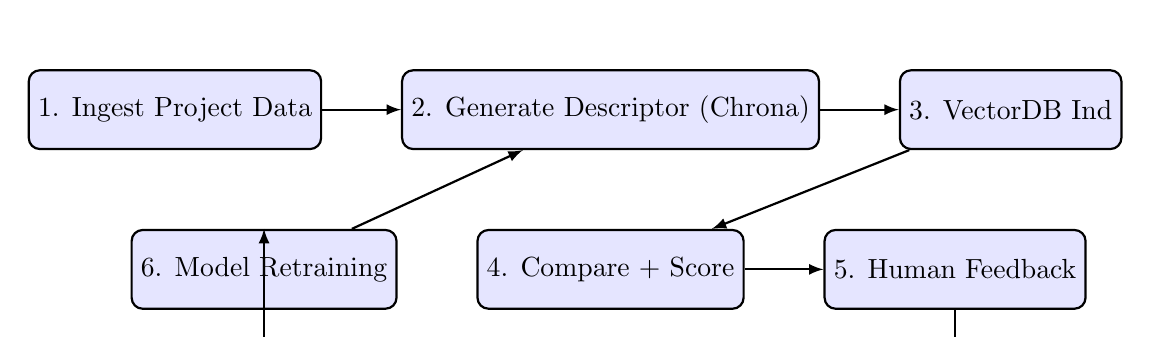
\begin{tikzpicture}[node distance=1cm, >=latex, thick]
\tikzstyle{block} = [rectangle, draw, fill=blue!10, rounded corners, minimum height=1cm, minimum width=2.5cm, text centered]
\tikzstyle{arrow} = [->, thick]

\node[block] (ingest) {1. Ingest Project Data};
\node[block, right=of ingest] (summarize) {2. Generate Descriptor (Chrona)};
\node[block, right=of summarize] (index) {3. VectorDB Ind};
\node[block, below=of summarize] (match) {4. Compare + Score};
\node[block, right=of match] (review) {5. Human Feedback};
\node[block, left=of match] (retrain) {6. Model Retraining};

\draw[arrow] (ingest) -- (summarize);
\draw[arrow] (summarize) -- (index);
\draw[arrow] (index) -- (match);
\draw[arrow] (match) -- (review);
\draw[arrow] (review.south) -- ++(0,-0.5) -| (retrain.north);
\draw[arrow] (retrain) -- (summarize);
\end{tikzpicture}
\end{center}

\section{Pilot Project Plan}

\subsection{Resources}
\begin{itemize}[leftmargin=2em]
    \item ~8 FTEs (engineers, analysts, PM)  
    \item Infrastructure budget: \$1.2--1.5M  
\end{itemize}

\section{Governance, Compliance, and Change Management}
\subsection{Governance Framework}
\begin{itemize}[leftmargin=2em]
    \item Transparency: All outputs auditable and explainable.  
    \item Accountability: Human validation remains final.  
    \item Control: Oversight board for model retraining, data ingestion, and external repository access.  
\end{itemize}

\subsection{Compliance \& IP Protection}
\begin{itemize}[leftmargin=2em]
    \item Private deployment; no third-party API exposure.  
    \item Projects classified by sensitivity (Public, Internal, Confidential, Restricted).  
    \item Legal review of open-source license compliance.  
\end{itemize}

\subsection{Change Management}
\begin{itemize}[leftmargin=2em]
    \item Executive sponsorship: CIO/CTO.  
    \item Divisional ambassadors to drive adoption.  
    \item Training for PMs to interpret descriptors and overlap scores.  
    \item Incentives for divisions demonstrating reuse and efficiency.  
\end{itemize}

\section{KPIs}
\subsection{Technical}
\begin{itemize}[leftmargin=2em]
    \item Descriptor consistency $\geq$ 85\%  
    \item Precision $\geq$ 75\%, Recall $\geq$ 70\%  
\end{itemize}

\subsection{Business}
\begin{itemize}[leftmargin=2em]
    \item 10--20\% of projects flagged as redundant  
    \item >5\% substitution with open-source  
    \item \$5M+ in identified cost savings  
\end{itemize}

\subsection{Adoption}
\begin{itemize}[leftmargin=2em]
    \item Reviewer acceptance $\geq$ 70\%  
    \item Division adoption $\geq$ 80\%  
\end{itemize}

\section{Business Case \& ROI}
\subsection{ROI Bar Chart}

\begin{center}
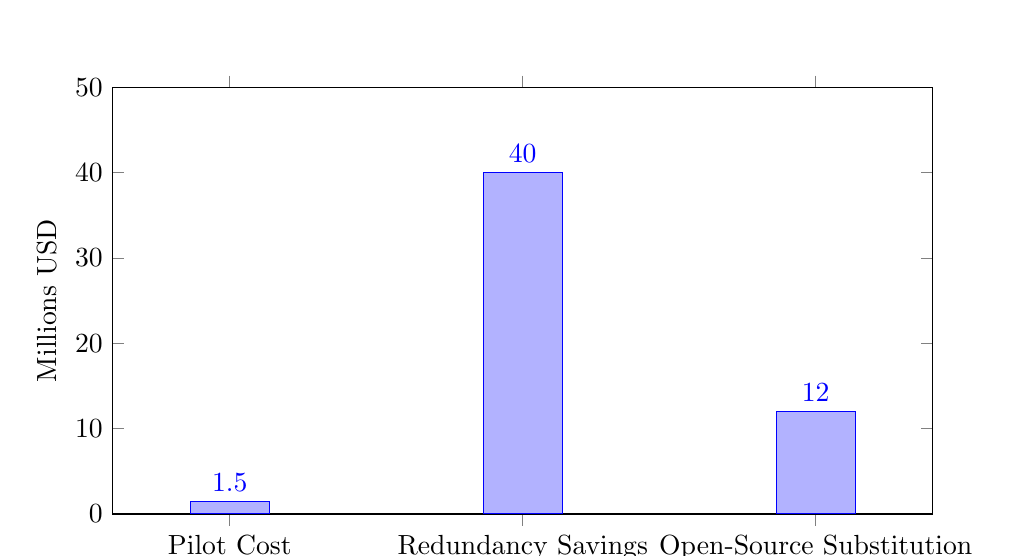
\begin{tikzpicture}
\begin{axis}[
    ybar,
    symbolic x coords={Pilot Cost, Redundancy Savings, Open-Source Substitution},
    xtick=data,
    ylabel={Millions USD},
    width=12cm,
    height=7cm,
    nodes near coords,
    nodes near coords align={vertical},
    bar width=1cm,
    ymin=0,
    ymax=50,
    enlarge x limits=0.2
]
\addplot coordinates {(Pilot Cost,1.5) (Redundancy Savings,40) (Open-Source Substitution,12)};
\end{axis}
\end{tikzpicture}
\end{center}

\subsection{Strategic Benefits}
\begin{itemize}[leftmargin=2em]
    \item Reduced redundancy and faster innovation cycles.  
    \item Optimized R\&D spend and better resource allocation.  
    \item Enhanced knowledge visibility across divisions.  
\end{itemize}

\subsection{ROI Estimate}
\begin{itemize}[leftmargin=2em]
    \item Avoided redundant spend: \$40M annually  
    \item Open-source substitution: \$10--15M  
    \item Pilot cost: \$1.5M  
    \item Estimated ROI: $>$20x within Year 1  
\end{itemize}

\section{Next Steps}
\begin{enumerate}[leftmargin=2em]
    \item Board approval for 3-month pilot funding  
    \item Select pilot divisions  
    \item Establish governance board  
    \item Launch Phase 1: Taxonomy \& ingestion pipeline 
\end{enumerate}

\section{Conclusion}
\textbf{Project Chronos: Insight Refined, Innovation Amplified} provides a strategic, high-ROI solution to enterprise project redundancy. Leveraging \textbf{Chrona}, the enterprise can save tens of millions annually, accelerate innovation, and transform how knowledge is reused across divisions.

\end{document}
